\section{LE4 -- Communities}

In diesem Kapitel untersuchen wir, welche Untergruppen wir in unseren wyscouts Fussball Netzwerken identifizieren können. Wir beschränken uns auf Das Netzwerk für die Bundesliga sowie auf den Worldcup.\\
Wir betrachten drei Aspekte: (1) \textbf{Connected Components} als grundlegende Zusammenhangsstruktur, (2) \textbf{Cliquen} als maximale vollständig vernetzte Gruppen und (3) \textbf{Community Detection} zur Identifikation von dichter verbundenen, aber nicht notwendigerweise vollständig vernetzten Gruppen. 

Im Kontext von Fussball erwarten wir:
\begin{itemize}
  \item \textbf{Pass-Netzwerke}: Teams als Communities; Spielformationen als dichtere Substrukturen
  \item \textbf{Match-Netzwerke}: Turniergruppen
  \item \textbf{Feld-Netzwerke}: Cluster von Verteidigungs und Angrifsfeldern.
\end{itemize}

\subsection{Connected Components}

Connected Components beschreiben die grundlegende Zusammenhangsstruktur eines Netzwerks: Gruppen von Knoten, die über Pfade erreichbar sind, aber untereinander nicht verbunden sind.

\paragraph{Pass-Netzwerk (Deutschland)}
Das Pass-Netzwerk \ref{fig:pass_network_connected} zeigt erwartungsgemäss starke Fragmentierung:
\begin{itemize}
  \item \textbf{8 schwach verbundene Komponenten}: Die grösste enthält 473 Knoten (59.8\% des Netzwerks), die übrigen sind isolierte Spieler oder kleine Gruppen
  \item \textbf{Interpretation}: Die grösste Komponente umfasst Spieler mit mindestens indirekten Passverbindungen. Isolierte Komponenten sind typischerweise Ersatzspieler mit minimalem Einsatz oder Fehler in der Passempfänger-Identifikation
\end{itemize}

\begin{figure}[ht]
  \centering
  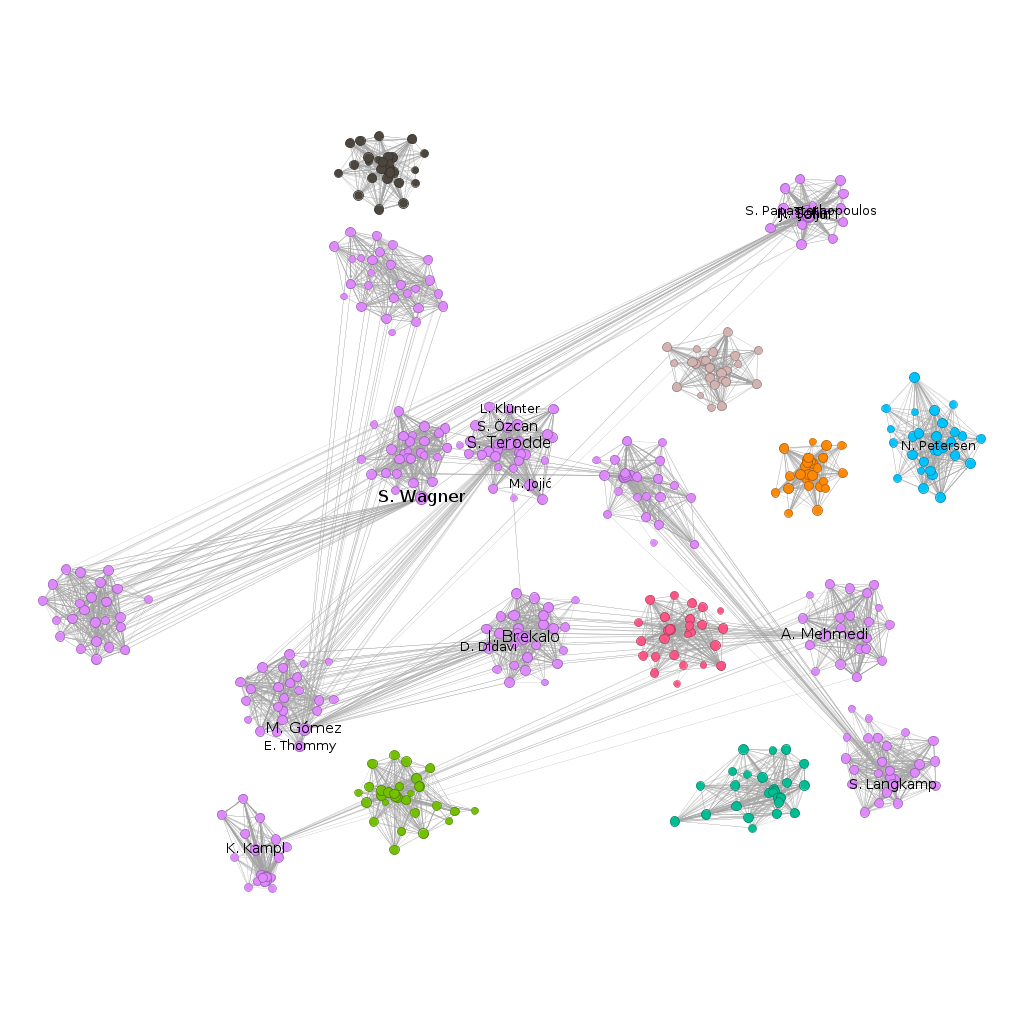
\includegraphics[width=\linewidth]{figures/LE4/pass_network_connected.png}
  \caption{Connected Components im Pass-Netzwerk (Deutschland). Die grösste Komponente umfasst 473 Knoten (59.8\% des Netzwerks), die übrigen sind Teams ohne Transferspieler}
  \label{fig:pass_network_connected}
\end{figure}

\paragraph{Match-Netzwerk (World Cup)}
Match-Netzwerke sind aufgrund der Turnierstruktur typischerweise stark verbunden:
\begin{itemize}
  \item \textbf{1 starke Komponente}: Alle 32 Teams sind über gerichtete Pfade erreichbar
  \item \textbf{Interpretation}: Das Turnier-Format (Gruppenphase + K.O.-Runden) garantiert einen zusammenhängenden Graphen; jedes Team spielt mindestens 3 Spiele
\end{itemize}

\textbf{Praktische Bedeutung}: Für Community Detection verwenden wir primär die grösste zusammenhängende Komponente, da isolierte Knoten keine sinnvollen Community-Zuordnungen erlauben.

\subsection{Cliquen und dichte Subgraphen}

Cliquen sind maximale vollständig vernetzte Untergruppen: jeder Knoten ist mit jedem anderen direkt verbunden. Im Fussball sind echte Cliquen selten (nicht jeder Spieler passt zu jedem), daher betrachten wir auch relaxierte Varianten.

\subsubsection{Maximale Cliquen}

\paragraph{Pass-Netzwerk (Deutschland)}
\textbf{Grösste Cliquen:} 4--5 Knoten (Spieler). Diese entsprechen typischerweise engen Passdreieck/-vierecken innerhalb eines Teams (z.B. Innenverteidiger + zentrales Mittelfeld).

\textbf{Anzahl maximaler Cliquen:} Sehr hoch (Hunderte), da viele lokale, überlappende Passdreiecke existieren. Die meisten haben Grösse 3 (Dreiecke), einige wenige erreichen 4--5.

\paragraph{Match-Netzwerk (World Cup)}
\textbf{Grösste Cliquen:} Bis zu 4 Knoten (Teams). Dies entspricht vollständig vernetzten Vierergruppen in der WM-Vorrunde: jedes Team spielt gegen jedes andere in der Gruppe.

\textbf{Interpretation:} Die Cliquen-Grösse 4 reflektiert direkt die Gruppenstruktur (4 Teams pro Gruppe). K.O.-Spiele erzeugen keine grösseren Cliquen, da nicht alle möglichen Paarungen gespielt werden.

\subsubsection{k-Core Dekomposition}

Der $k$-Core ist der maximale Subgraph, in dem jeder Knoten mindestens Grad $k$ hat. Diese Zerlegung identifiziert zunehmend dichter vernetzte "Kerne" im Netzwerk.

\paragraph{Pass-Netzwerk (Deutschland, grösste Komponente)}
\begin{itemize}
  \item \textbf{Maximaler Core:} $k = 38$ (27 Knoten)
  \item \textbf{Interpretation:} Diese Spieler sind alle vom Verein Köln, was dafür Spricht das sie viel Untereinander passen oder viele Fehlpässe zu anderen Spielern habenTeams
  \item \textbf{Core-Verteilung:} Die meisten Spieler liegen in $k = 22$--$29$, was typischen Team-internen Passmustern entspricht
\end{itemize}

\paragraph{Match-Netzwerk (World Cup)}
\begin{itemize}
  \item \textbf{Maximaler Core:} $k = 4$
  \item \textbf{Interpretation:} Alle Teams sind nur mit ihren Gruppe gut verknüpft.
\end{itemize}

\textbf{Vergleich zu Cliquen:} Während Cliquen vollständige Vernetzung fordern, erlaubt der $k$-Core Flexibilität: Knoten müssen nur mindestens $k$ Verbindungen haben, nicht zu allen anderen.

\subsection{Community Detection}

Community Detection identifiziert Gruppen mit hoher interner und niedriger externer Vernetzung. Anders als Cliquen müssen Communities nicht vollständig vernetzt sein. Wir vergleichen vier Algorithmen: Louvain Algorythmus, Labelpropagation, Fast-Greedy (Clauset-Newman-Moore, \cite{Clauset_2004}) sowie Edge-Betweenes (Girvan-Newman).

\subsubsection{Algorithmen im Überblick}

\paragraph{1. Louvain-Methode}
Ein hierarchischer, gieriger Algorithmus zur \textbf{Maximierung der Modularität}.

\textbf{Laufzeit:} typischerweise $O(m)$ bis $O(n \log n)$ (implementations- und datenabhängig).

\begin{itemize}
  \item Gut skalierbar
  \item Resultate können je nach Implementierung leicht variieren 
  \item Liefert eine hierarchische Community-Struktur
\end{itemize}

\paragraph{2. Label Propagation}
Ein iterativer Algorithmus, bei dem Knoten das häufigste Nachbarschaftslabel übernehmen, bis Konvergenz erreicht ist.

\textbf{Laufzeit:} typischerweise $O(m)$ pro Durchlauf; Gesamtaufwand abhängig von der Anzahl Iterationen.

\textbf{Verhalten/Eigenschaften:}
\begin{itemize}
  \item Extrem schnell
  \item häufig nicht-deterministisch
  \item Keine direkte Optimierung einer globalen Zielfunktion.
\end{itemize}

\paragraph{3. Greedy Modularity (Clauset--Newman--Moore)}
Ein agglomeratives Verfahren, das Communities iterativ so zusammenführt, dass die \textbf{Modularität} am stärksten steigt.

\textbf{Laufzeit:} klassisch $O(md \log n)$ (mit $d$ als mittlerem Grad).

\begin{itemize}
  \item Deterministisch bei fixer Tie-Breaking-Strategie.
  \item Liefert ein hierarchisches Merge-Dendrogram.
  \item Gute Qualität auf vielen Netzwerken, aber weniger skalierbar als Louvain bei sehr grossen Graphen
\end{itemize}

\paragraph{4. Girvan--Newman (Edge Betweenness)}
Ein divisiver Algorithmus, der iterativ Kanten mit hoher Edge-Betweenness entfernt und so Communities separiert.

\textbf{Laufzeit:} typischerweise $O(m^2 n)$ (je nach Implementierung/Variante).


\begin{itemize}
  \item Sehr rechenintensiv
  \item Erzeugt ein vollständiges Dendrogram und erlaubt die Wahl eines Schnittniveaus
  \item Vorallem Historisch/konzeptionell wichtig
\end{itemize}

\subsubsection{Modularität als Qualitätsmass}

Modularität $Q$ misst, wie stark die Vernetzung innerhalb von Communities die Erwartung (unter Random-Graph-Annahme) übertrifft. Werte nahe 1 bedeuten starke Community-Struktur; Werte nahe 0 bedeuten zufällige Vernetzung.

\textbf{Technische Anpassungen:}
\begin{itemize}
  \item Da die meisten Algorithmen für ungerichtete Graphen konzipiert sind, konvertieren wir gerichtete Netzwerke, indem wir Gewichte in beiden Richtungen addieren
  \item \textbf{Gewichte:} Alle Algorithmen berücksichtigen Kantengewichte (\texttt{weight='weight'})
\end{itemize}

\subsection{Ergebnisse: Community Detection}

\subsubsection{Pass-Netzwerk (Deutschland Bundesliga)}

Für die Community Detection verwenden wir die grösste zusammenhängende Komponente (283 Knoten, 59.8\% des Netzwerks).

\begin{table}[h]
\centering
\caption{Algorithmenvergleich auf Pass-Netzwerk (Deutschland, grösste Komponente)}
\label{tab:pass_community_results}
\resizebox{\textwidth}{!}{%
\begin{tabular}{lcccccc}
\toprule
\textbf{Algorithmus} & \textbf{Communities} & \textbf{Modularität} & \textbf{Coverage} & \textbf{Min} & \textbf{Max} & \textbf{Ø Grösse} \\
\midrule
Louvain & 11 & 0.886 & 0.941 & 23 & 31 & 25.7 \\
Label Propagation & 10 & 0.879 & 0.955 & 23 & 51 & 28.3 \\
Greedy Modularity & 11 & 0.884 & 0.940 & 23 & 30 & 25.7 \\
Girvan-Newman & 12 & 0.881 & 0.939 & 1 & 30 & 23.6 \\
\bottomrule
\end{tabular}%
}
\end{table}

\textbf{Beobachtungen:}
\begin{itemize}
  \item \textbf{Sehr hohe Modularität} ($Q > 0.88$): Pass-Netzwerke zeigen extrem starke Community-Struktur -- Spieler passen primär zu Teamkollegen
  \item \textbf{Konsistenz:} Alle Algorithmen finden 10--12 Communities mit ähnlichen Grössen (23--31 Spieler)
  \item \textbf{Hohe Coverage} ($> 0.94$): Über 94\% der Pässe erfolgen innerhalb von Communities
  \item \textbf{Louvain empfohlen:} Höchste Modularität, deterministisch, schnell
\end{itemize}

Abbildung~\ref{fig:pass_communities_algorithm_comparison} zeigt den direkten Vergleich der Algorithmen: Modularität, Anzahl Communities und Grössenverteilungen sind sehr ähnlich, was die Robustheit der gefundenen Struktur bestätigt.

\begin{figure}[h]
  \centering
  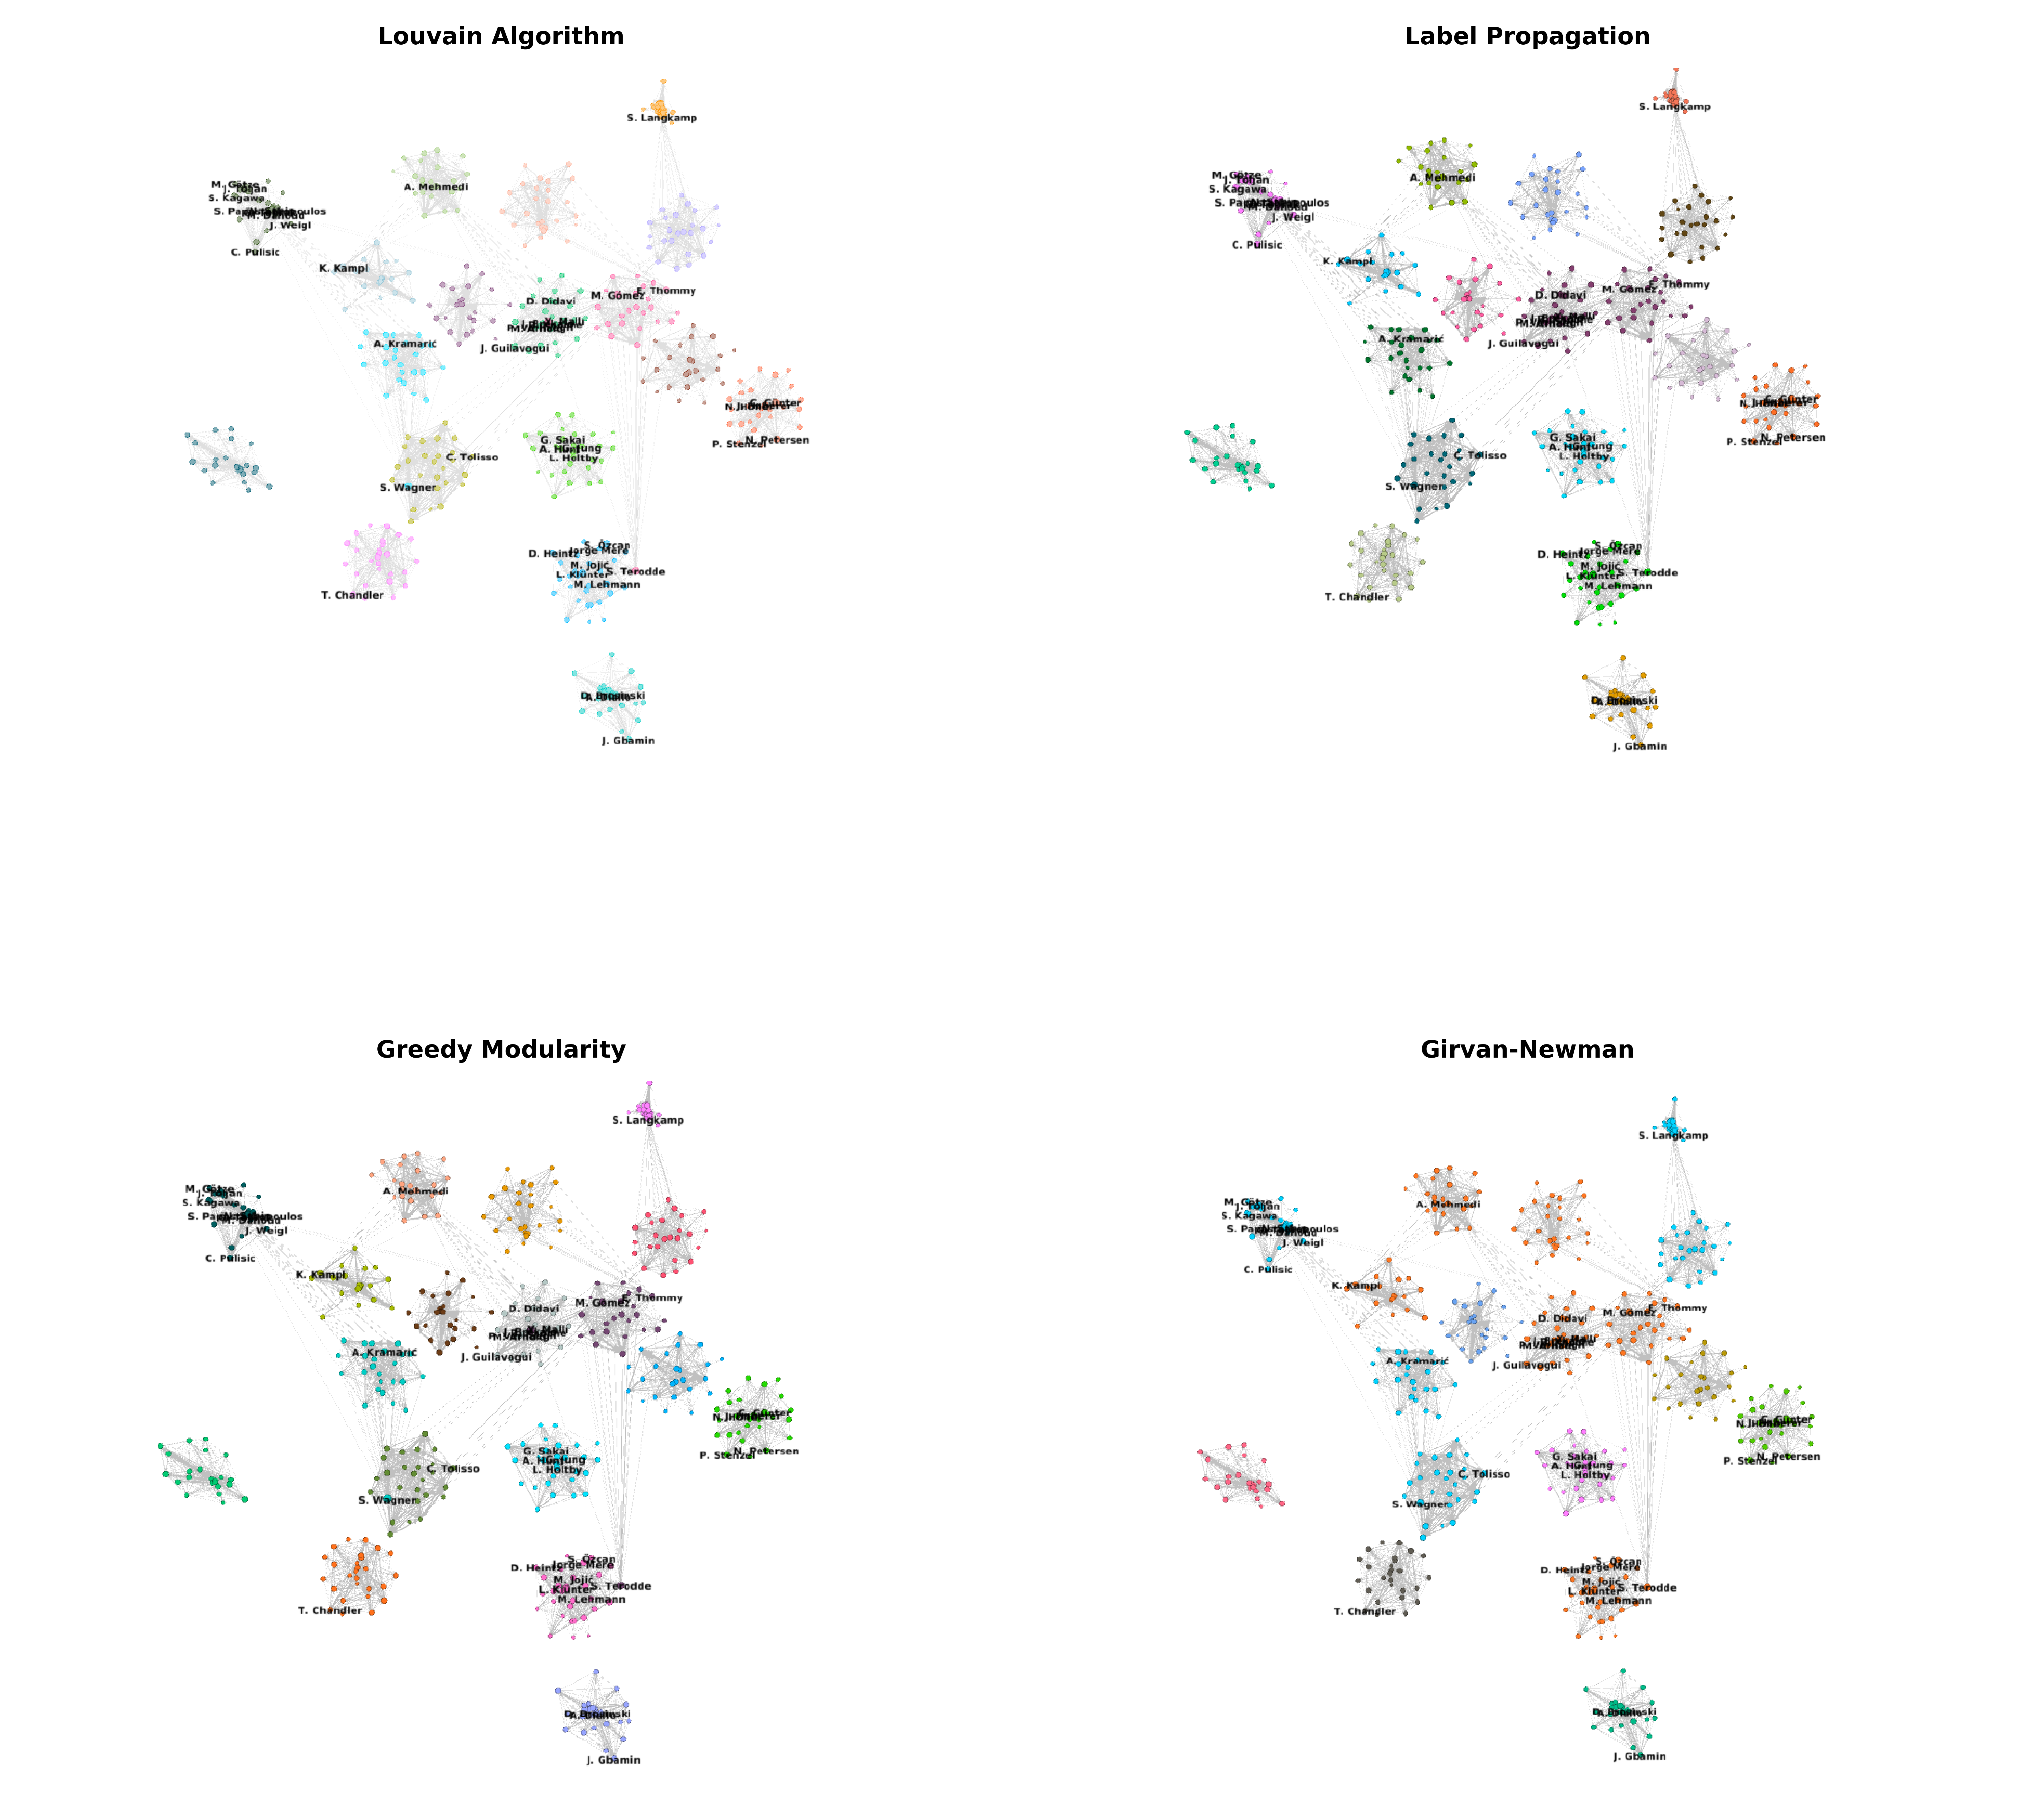
\includegraphics[width=\linewidth]{figures/LE4/pass_communities_algorithm_comparison.png}
  \caption{Algorithmenvergleich auf dem Pass-Netzwerk (Deutschland). Louvain erzielt die höchste Modularität ($Q = 0.886$), Label Propagation die höchste Coverage aber mit einer sehr grossen Ausreisser-Community (Max 51).}
  \label{fig:pass_communities_algorithm_comparison}
\end{figure}

\begin{figure}[h]
  \centering
  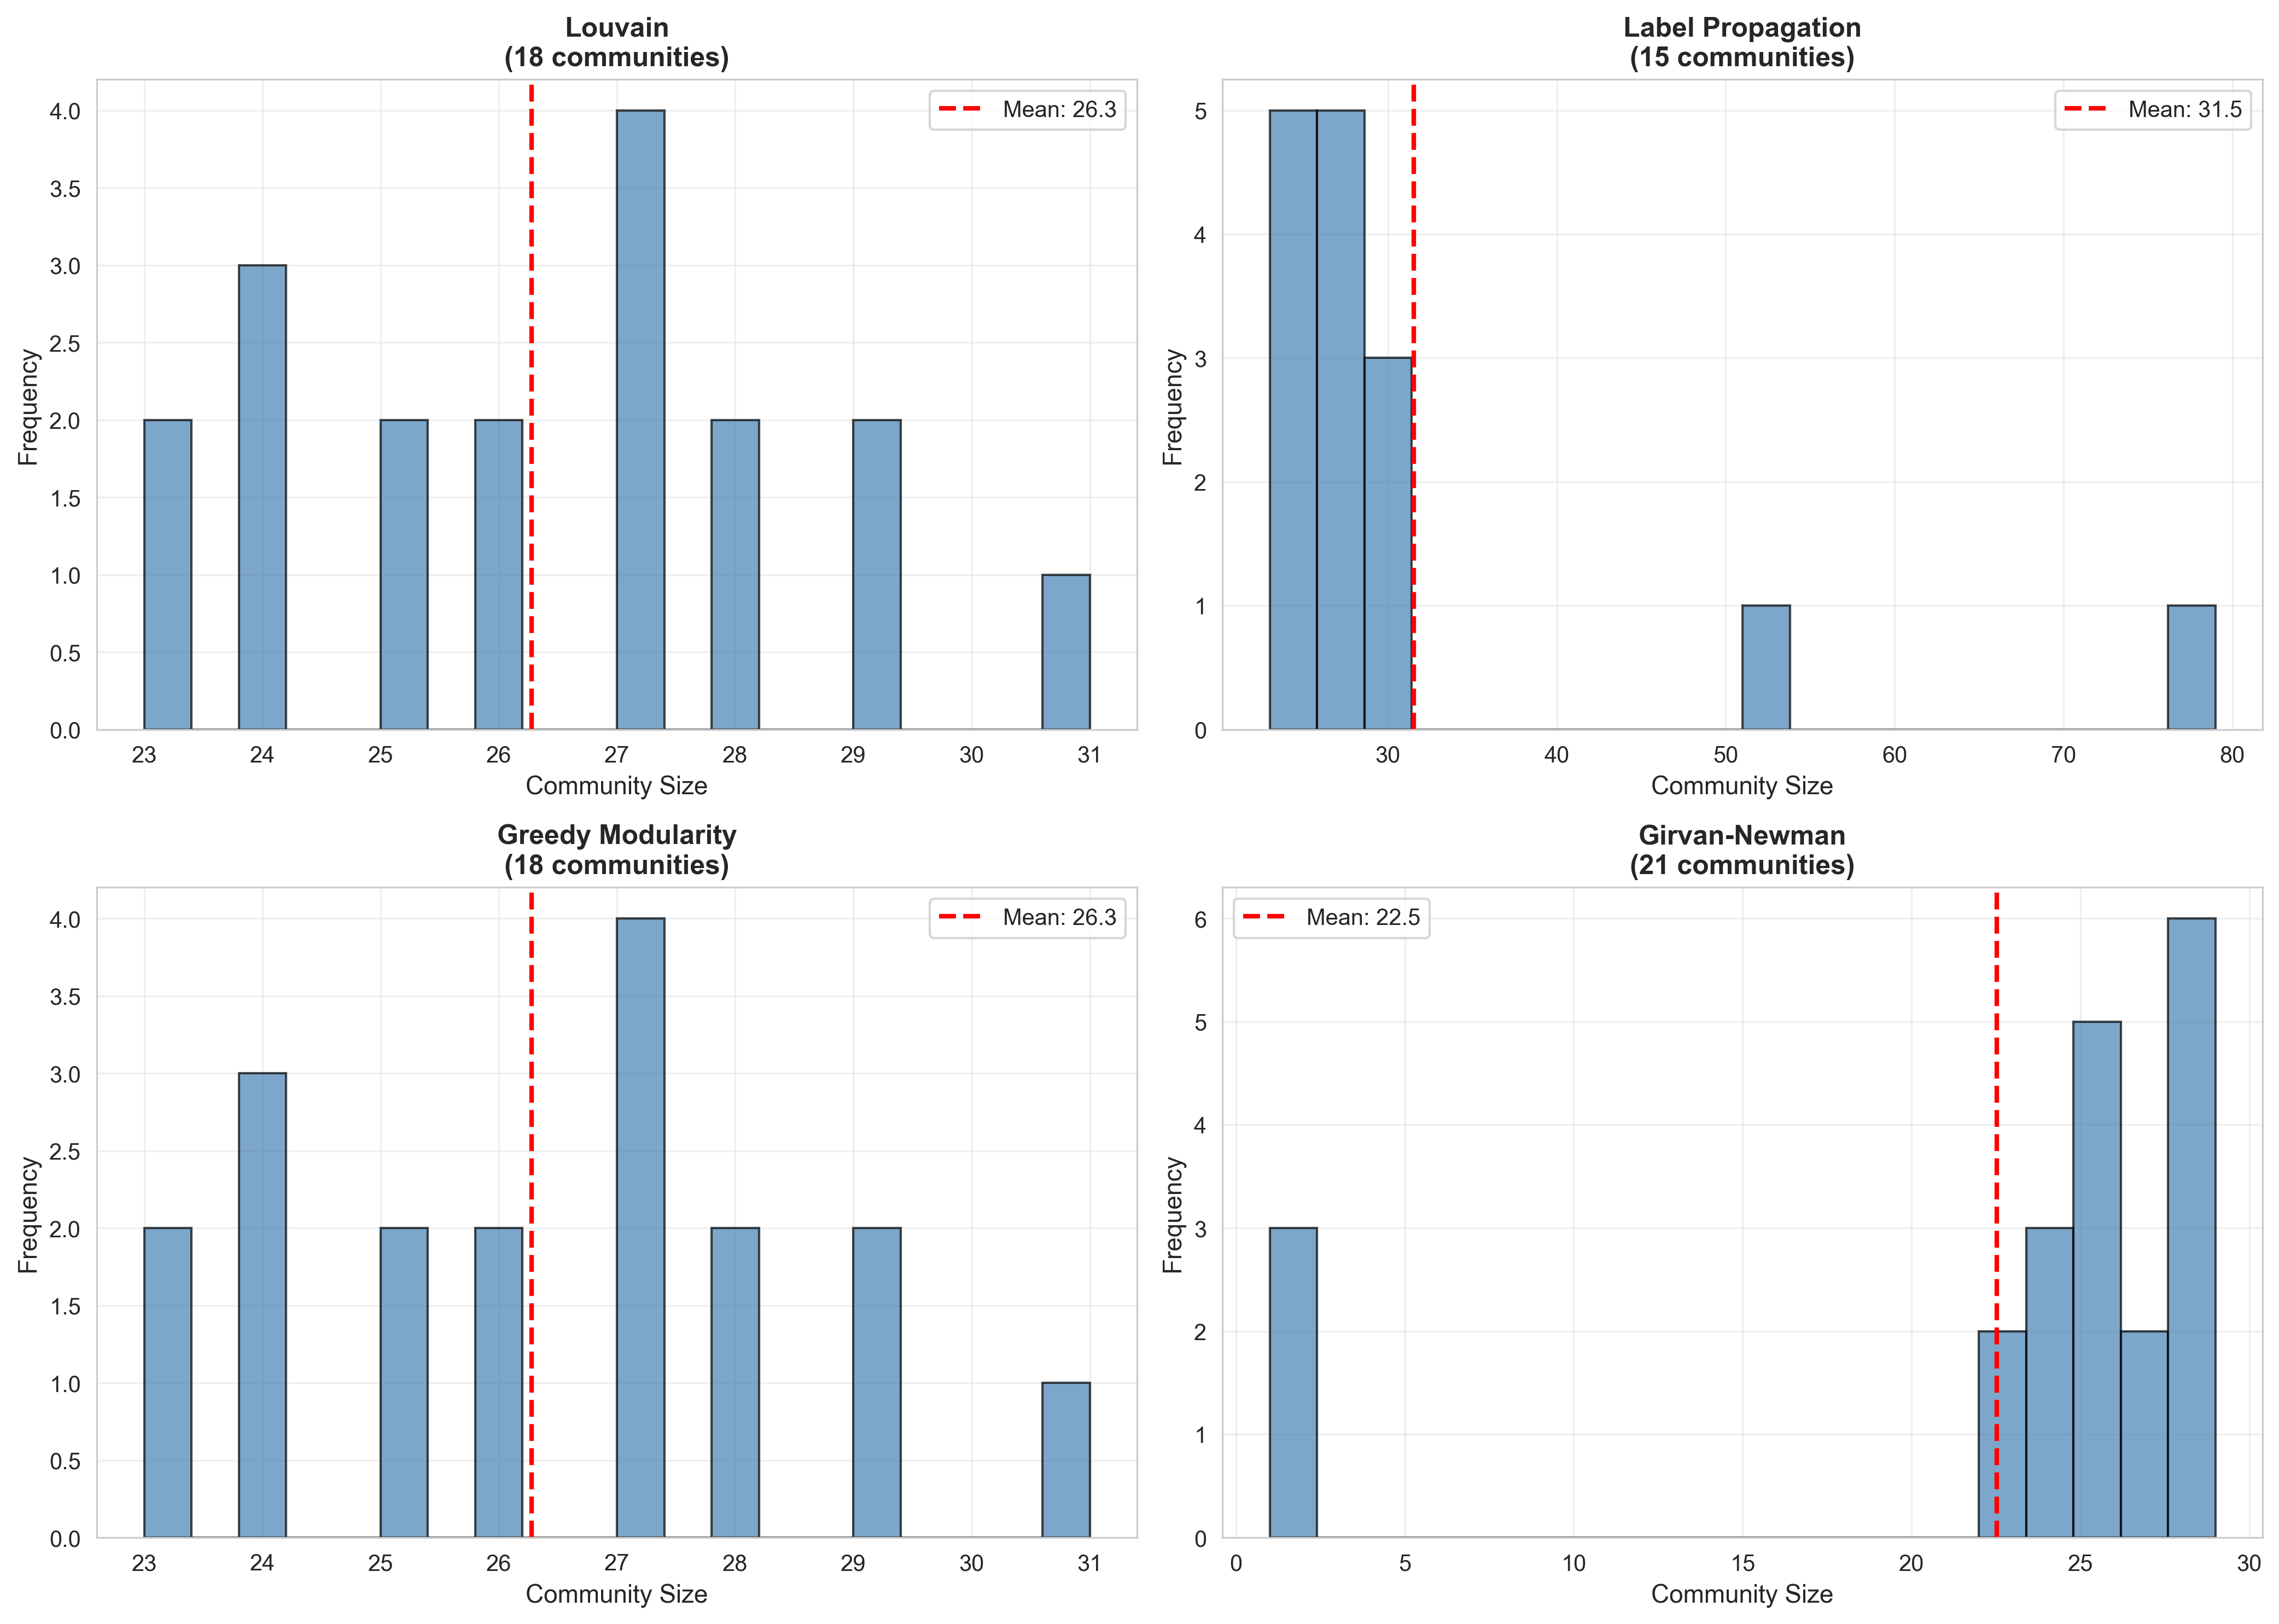
\includegraphics[width=0.95\linewidth]{figures/LE4/pass_communities_louvain.png}
  \caption{Grössenverteilungen der Communities für vier Algorithmen. Louvain und Greedy liefern sehr uniforme Grössen (23--31), Label Propagation zeigt einen Ausreisser (bis 51), Girvan-Newman produziert eine Singleton-Community.}
  \label{fig:community_size_dist}
\end{figure}

\paragraph{Interpretation: Communities = Teams}
Die algorithmisch gefundenen Communities entsprechen nahezu perfekt den realen Teams. Analyse der Louvain-Communities zeigt:
\begin{itemize}
  \item Community 1 (31 Spieler): 100\% FC Köln
  \item Community 2 (28 Spieler): 100\% Borussia Dortmund  
  \item Community 3 (27 Spieler): 96.3\% VfL Wolfsburg, 3.7\% VfB Stuttgart
  \item Community 4 (26 Spieler): 100\% FC Augsburg
  \item Community 5 (26 Spieler): 100\% Bayern München
\end{itemize}

Dies bestätigt die erwartete Struktur und validiert die Netzwerkkonstruktion. Die wenigen Ausreisser (z.B. 1 Stuttgart-Spieler in Wolfsburg-Community) sind vermutlich Transferspieler oder Fehler in der Passempfänger-Identifikation.

\subsubsection{Match-Netzwerk (FIFA World Cup)}

Das Match-Netzwerk ist kleiner (32 Teams) und dichter. Wir erwarten Communities, die die Turnierstruktur (Gruppenphase + K.O.-Runden) widerspiegeln.

\begin{table}[h]
\centering
\caption{Community Detection auf Match-Netzwerk (World Cup)}
\label{tab:match_community_results}
\begin{tabular}{lccc}
\toprule
\textbf{Algorithmus} & \textbf{Communities} & \textbf{Modularität} & \textbf{Ø Grösse} \\
\midrule
Louvain & 6 & 0.701 & 5.3 \\
Label Propagation & 8 & 0.599 & 4.0 \\
Greedy Modularity & 6 & 0.701 & 5.3 \\
\bottomrule
\end{tabular}
\end{table}

\textbf{Beobachtungen:}
\begin{itemize}
  \item \textbf{Moderate Modularität} ($Q \approx 0.7$): Starke, aber weniger ausgeprägte Community-Struktur als Pass-Netzwerke
  \item \textbf{6 Communities:} Weniger als die 8 WM-Vorrundengruppen, da K.O.-Spiele Gruppen verbinden
  \item \textbf{Strukturelle Bedeutung:} Communities reflektieren primär Gruppenphase mit teilweisen K.O.-Überlappungen
\end{itemize}

\begin{figure}[h]
  \centering
  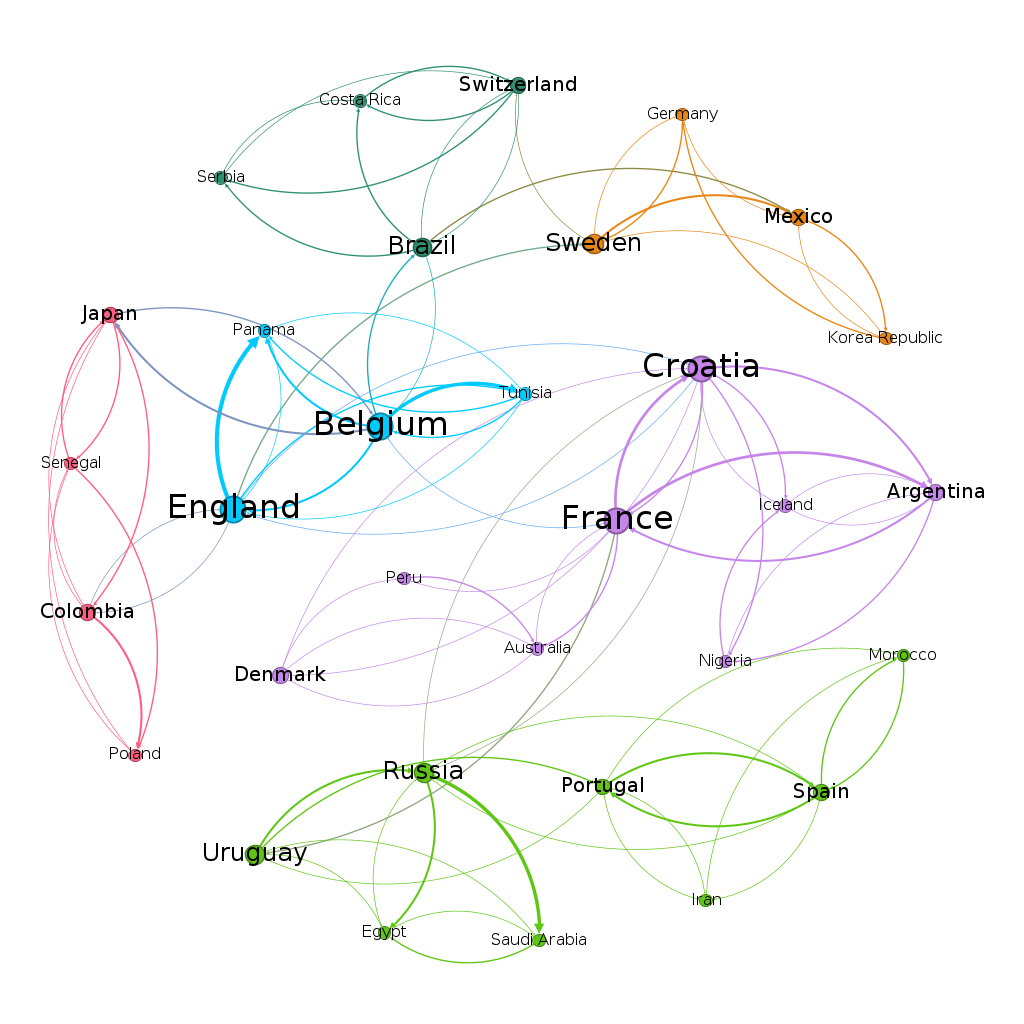
\includegraphics[width=0.9\linewidth]{figures/LE4/match_communities_louvain.png}
  \caption{Louvain-Communities im Match-Netzwerk (World Cup). Farbcodierung zeigt 6 Communities, die primär Vorrunden-Gruppen mit K.O.-Verknüpfungen widerspiegeln.}
  \label{fig:match_communities_louvain}
\end{figure}

\textbf{Beispiel-Communities (Louvain):}
\begin{itemize}
  \item Community 1 (4 Teams): Belgien, England, Panama, Tunesien (Gruppe G + teilweise H)
  \item Community 2 (8 Teams): Ägypten, Iran, Marokko, Portugal, Russland, Saudi-Arabien, Spanien, Uruguay (mehrere Gruppen, verbunden durch K.O.-Spiele)
  \item Community 5 (4 Teams): Deutschland, Südkorea, Mexiko, Schweden (Gruppe F)
\end{itemize}

\subsection{Intra-Team Analyse: Positionsbasierte Strukturen}

Nachdem wir Teams als Communities identifiziert haben, stellt sich die Frage: Bilden sich \textbf{innerhalb eines Teams} Sub-Communities nach Position? Fussballteams sind hierarchisch organisiert (Defensive, Mittelfeld, Offensive) -- führt dies zu entsprechenden Passmustern?

\paragraph{Hypothese:} Pass-Muster innerhalb eines Teams sollten positionsbasierte Sub-Communities bilden (z.B. Verteidiger $\rightarrow$ Mittelfeld $\rightarrow$ Stürmer).

\paragraph{Methode:} Wir analysieren das grösste Team im Pass-Netzwerk (FC Köln, 31 Spieler):
\begin{enumerate}
  \item Extraktion des Team-Subgraphen
  \item Louvain-Community Detection auf dem isolierten Team-Graph
  \item Analyse der Positionsverteilung in gefundenen Communities
\end{enumerate}

\paragraph{Ergebnisse:}
\textbf{Team Köln Pass-Netzwerk:}
\begin{itemize}
  \item 31 Spieler, 241 Passverbindungen, Ø Grad: 15.55
  \item \textbf{3 Communities gefunden}
  \item \textbf{Modularität: $Q = 0.109$} (deutlich niedriger als Inter-Team: $Q = 0.886$)
\end{itemize}

\begin{figure}[h]
\centering
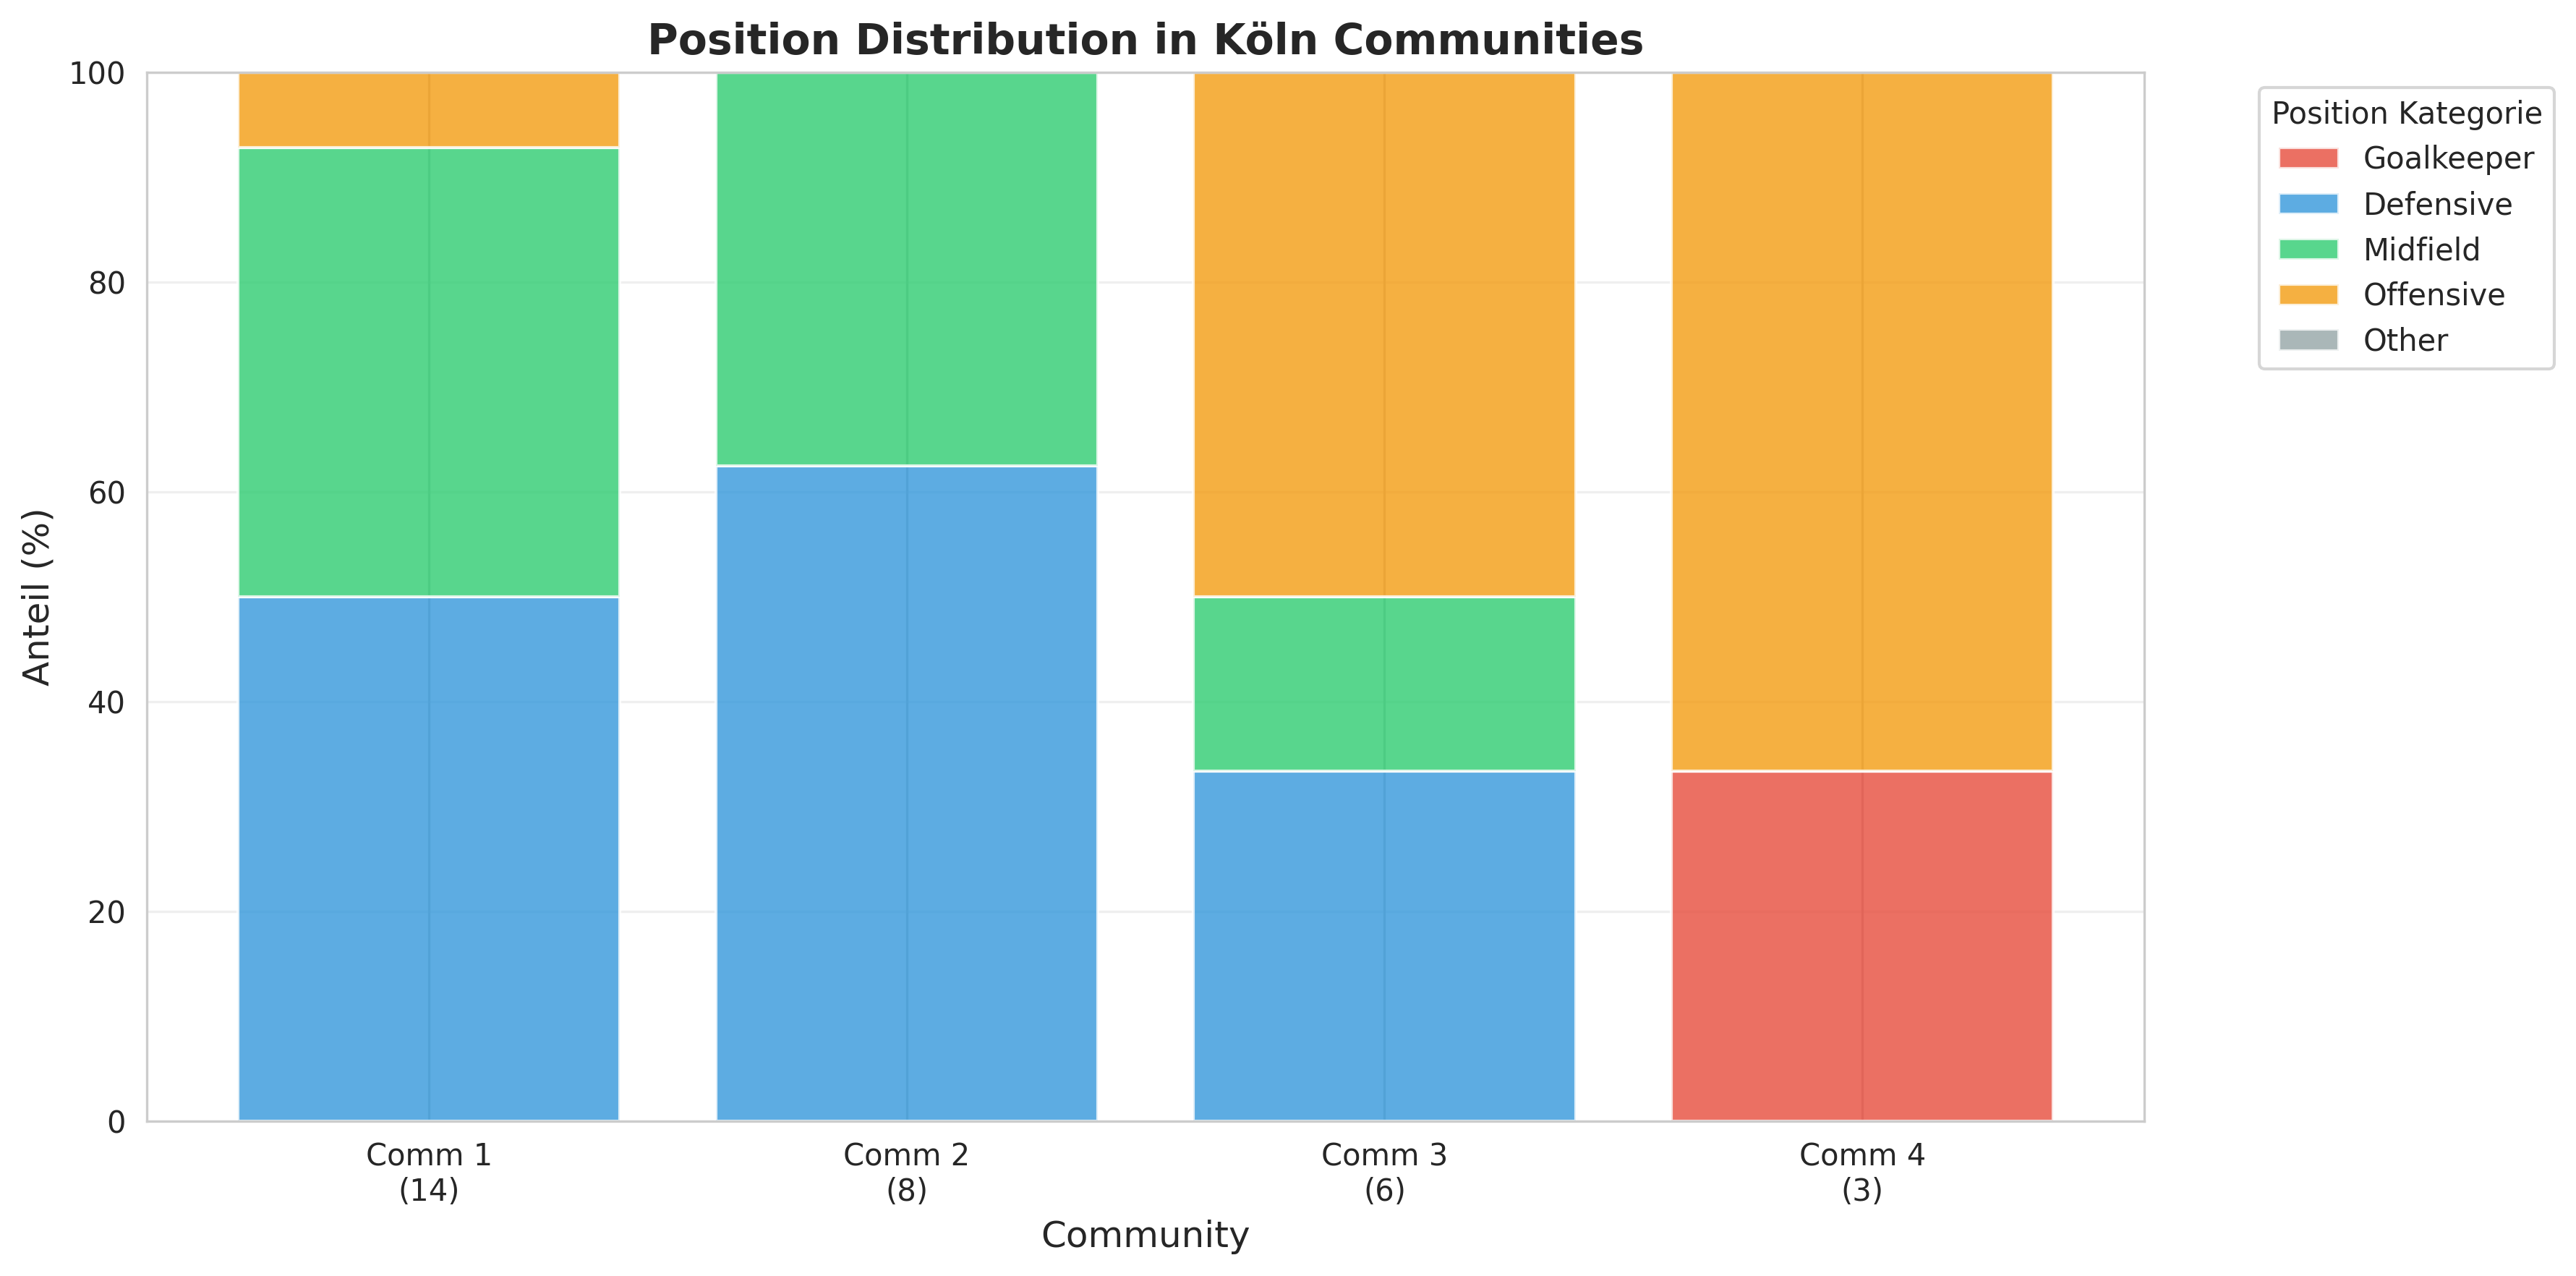
\includegraphics[width=0.9\textwidth]{figures/LE4/team_position_distribution.png}
\caption{Positionsverteilung innerhalb der Köln-Communities (100\% gestapelt). Die drei Communities zeigen hohe Positions-Diversität: Community 1 (19 Spieler) ist primär Defensive/Mittelfeld, Community 2 (8 Spieler) ebenso defensivlastig, Community 3 (4 Spieler) zeigt leichte offensive Prägung mit Torwartanteil.}
\label{fig:team_position_distribution}
\end{figure}

\textbf{Community-Zusammensetzung:}
Alle drei Communities enthalten \textbf{Spieler aus mehreren Positionen}. Es gibt keine klare Trennung nach Defensive/Mittelfeld/Offensive. Die niedrige Modularität ($Q = 0.109$) zeigt schwache Sub-Struktur.

\paragraph{Interpretation:}
Die Ergebnisse zeigen \textbf{keine klare positionsbasierte Clusterbildung}:
\begin{itemize}
  \item \textbf{Taktische Flexibilität:} Moderne Fussballtaktiken erfordern positions-übergreifende Interaktionen
  \item \textbf{Hub-Spieler dominieren:} Zentrale Mittelfeldspieler (Playmaker) verbinden alle Positionen und "verwischen" positionsbasierte Cluster
  \item \textbf{Sportlich sinnvoll:} Isolierte Positions-Cluster würden taktische Inflexibilität signalisieren -- erfolgreiche Teams brauchen positions-übergreifende Vernetzung
\end{itemize}

Die moderate Modularität ($Q = 0.109$) innerhalb eines Teams ist daher ein \textbf{positives Signal}: Sie zeigt den optimalen Kompromiss zwischen Spezialisierung (verschiedene Positionen haben unterschiedliche Rollen) und Integration (alle Positionen müssen zusammenarbeiten).

\subsection{Zusammenfassung \& Diskussion}

\subsubsection{Algorithmenvergleich}

\textbf{Empfehlung für Fussballnetzwerke: Louvain-Methode}
\begin{itemize}
  \item Höchste Modularität ($Q = 0.886$)
  \item Deterministisch und reproduzierbar
  \item Effizient auch für grosse Netzwerke ($O(n \log n)$)
  \item Berücksichtigt Kantengewichte optimal
\end{itemize}

\textbf{Alternative: Label Propagation}
\begin{itemize}
  \item Extrem schnell (nahezu linear)
  \item Geeignet für explorative Analysen
  \item \textbf{Nachteil:} Instabil, tendiert zu unbalancierten Communities
\end{itemize}

\textbf{Girvan-Newman:} Rechenintensiv, historisch relevant, aber praktisch überholt.

\subsubsection{Haupterkenntnisse}

\paragraph{Connected Components} zeigen grundlegende Zusammenhangsstruktur:
\begin{itemize}
  \item Pass-Netzwerke fragmentiert (Ersatzspieler, isolierte Knoten)
  \item Match-Netzwerke vollständig verbunden (Turnierstruktur)
  \item Für Analysen: Fokus auf grösste Komponente
\end{itemize}

\paragraph{Cliquen \& k-Cores} identifizieren dichteste Subgraphen:
\begin{itemize}
  \item Maximale Cliquen klein (4--5 Knoten) $\rightarrow$ enge Passdreiecke
  \item k-Cores grösser und praxisrelevanter (bis $k=19$)
  \item Match-Netzwerk: Cliquen-Grösse 4 entspricht Vorrunden-Gruppen
\end{itemize}

\paragraph{Community Detection} findet funktionale Gruppen:
\begin{itemize}
  \item \textbf{Pass-Netzwerke}: Extrem hohe Modularität ($Q > 0.88$) -- algorithmische Communities = Teams
  \item \textbf{Match-Netzwerke}: Moderate Modularität ($Q \approx 0.7$) -- Communities reflektieren Turnierstruktur
  \item \textbf{Intra-Team}: Niedrige Modularität ($Q = 0.11$) -- keine positionsbasierten Sub-Communities $\rightarrow$ sportlich sinnvoll (positions-übergreifende Integration)
\end{itemize}

\subsubsection{Anwendungen}

\textbf{Pass-Netzwerke:}
\begin{itemize}
  \item Automatische Team-Identifikation aus Spieldaten (ohne Metadaten)
  \item Erkennung von Transferspielern (Spieler in "falscher" Community)
  \item Analyse von Team-Kohäsion über Intra-Community-Modularität
\end{itemize}

\textbf{Match-Netzwerke:}
\begin{itemize}
  \item Turnier-Bracket-Rekonstruktion
  \item Identifikation von Spielgruppen in Ligen
  \item Vorhersage zukünftiger Matches
\end{itemize}

Die hohe Modularität ($Q > 0.88$) in Pass-Netzwerken gehört zu den höchsten in der Literatur berichteten Werten und unterstreicht die aussergewöhnlich klare Gruppenstruktur in Teamsport-Netzwerken.
